\documentclass[12pt]{article}

\usepackage{graphicx}
\usepackage{titlesec}
\usepackage{xcolor}
\usepackage{enumitem}
\usepackage{subcaption}
\usepackage{float}
\usepackage{placeins}
\usepackage[none]{hyphenat}
\usepackage[most]{tcolorbox}
\usepackage[italian]{babel}
\usepackage[a4paper, margin=75pt]{geometry}
\usepackage[colorlinks=true, linkcolor=black]{hyperref}

\graphicspath{{images/}}
\setlist{itemsep=2pt}
\definecolor{greenpastel}{RGB}{180, 230, 180}
\tcbset{
  myboxstyle/.style={
    colback=white,
    coltitle=black,
    fonttitle=\bfseries,
    colframe=greenpastel
  }
}

\newcounter{definition}[section]
\renewcommand{\thedefinition}{\thesection.\arabic{definition}}
\newtcolorbox{definition}[1][]{
  myboxstyle,
  colframe=greenpastel,
  boxed title style={colback=greenpastel},
  before title={\refstepcounter{definition}},
  title={Definizione \thedefinition: #1}
}


\titleformat{\section}
  [block]
  {\raggedleft\LARGE\bfseries}
  {\textcolor{gray}{\scalebox{5}{\thesection}}}
  {0pt}
  {\\[3pt]}

\titlespacing*{\section}
  {0pt}   % rientro sinistro
  {0pt}   % spazio prima della sezione
  {30pt}  % spazio dopo la sezione


\begin{document}
  % --- Copertina ---
  \begin{titlepage}
      \centering

      % --- Logo Sapienza ---
      
\includegraphics[width=0.95\textwidth]{logo_sapienza.png}
      
      \vspace*{\stretch{0.2}}
      
      % --- Dati Sapienza ---
      {\LARGE "Sapienza" Università di Roma}\\[3pt]
      {\Large Ingegneria dell'Informazione, Informatica e Statistica}\\[3pt]
      {\large Dipartimento di Informatica}\\[3pt]
      
      % --- Spazio vuoto ---
      \vspace*{\stretch{1}}
      
      % --- Titolo ---
      \hrulefill\\
      \vspace{15pt}
      \textbf{\huge Programmazione WEB}\\
      \vspace{7pt}
      \hrulefill\\
      
      % --- Spazio vuoto ---
      \vspace*{\stretch{2}}
      
      % --- Autore ---
      \textit{\Large Autore}\\[3pt]
      {\Large Vincenzo Bova}\\
      
      % --- Spazio vuoto ---
      \vspace*{\stretch{1}}

      % --- Data ---
      {\large A.A. 2025/2026}\\
  \end{titlepage}

  % --- Indice ---
  \newpage
  \tableofcontents

  % --- Introduzione a Git ---
  \newpage
  \section{Introduzione a Git}
    \subsection{Sistemi di versionamento}
    Durante lo sviluppo di un progetto c'è spesso la necessità di effettuare revisioni, correzioni o modifiche ai file che lo compongono.
    \begin{figure}[H]
        \centering
        
\includegraphics[width=0.5\textwidth]{introduzione_a_git/no_git_example.png}
    \end{figure}
    Gestire ciò creando ogni volta nuovi file, tuttavia, comporta evidenti problemi:
    \begin{itemize}
      \item \textbf{Duplicazione del contenuto:} che rende il sistema inefficiente e aumenta la difficoltà nel mantenere integrità;
      \item \textbf{Assenza di Naming Convention:} che rende impossibile risalire ad uno storico delle modifiche;
      \item \textbf{Autori incerti};
      \item ...
    \end{itemize}
    \begin{samepage}
      Per ovviare a ciò sono stati creati i \textbf{sistemi di versionamento} (git, csv, mercurial, svn...), i quali offrono vari benefici:
      \begin{itemize}
        \item \textbf{Gestione delle versioni:} il sistema si occupa automaticamente di etichettare le varie versioni in modo consistente;
        \item \textbf{Tracciamento delle mofiche:} è possibile accedere ad uno storico delle modifiche effettuate;
        \item \textbf{Presenza di metadati:} ogni modifica ha un autore, una data...;
        \item \textbf{Creazione di linee di sviluppo parallele:} è possibile creare una versione parallela del codice per non modificare la versione principale, e poi riunirle integrando i cambiamenti;
        \item \textbf{Sincronizzazione tra computer:} il sistema consente di mantenere il progetto allineato tra più computer.
      \end{itemize}
    \end{samepage}

    \subsection{Git}
    Git è un sistema di versionamento distribuito e veloce, creato nel 2005 e capace di gestire progetti di grandi dimensioni.
    Si basa su un design semplice e utilizza DAG (\textit{Directed Acyclic Graph}) e Merkle trees come strutture dati.
    \begin{definition}[Repository]
      È un insieme di commit, branch e tag.\\
      Per semplicità assumiamo che un progetto equivale ad un repository.
    \end{definition}
    \begin{definition}[Working copy]
      È l'insieme dei file tracciati nella copia locale del repository.\\
      Quando creiamo un nuovo file non sarà ancora tracciato e bisognerà quindi aggiungerlo, quando invece modifichiamo un file già tracciato (\textit{update}) stiamo aggiornando la working copy.
    \end{definition}
    
    \subsubsection{Commit}
    Un commit è un'istantanea del repository in un determinato momento.\\
    Viene identificato dallo \textbf{SHA1} del commit stesso e contiene diversi campi:
    \begin{itemize}
      \item data + autore, data + commiter
      \item commento \textbf{obbligatorio}
      \item 0,1 o più genitori
      \item tree: hash di tutti i file nel commit
    \end{itemize}
    \begin{minipage}{\textwidth}
      In particolare il commit può contenere un sottoinsieme delle modifiche (anche ad un singolo file), le quali devono essere aggiunte alla staging area dei cambiamenti.
      \begin{figure}[H]
        \centering
        \begin{subfigure}{0.49\textwidth}
          \centering
          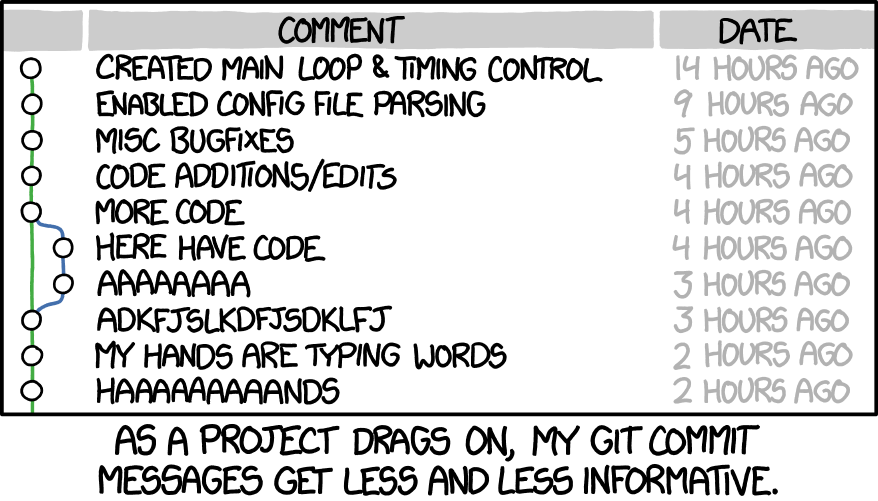
\includegraphics[height=4cm]{introduzione_a_git/git_commit.png}
        \end{subfigure}
        \hfill
        \begin{subfigure}{0.49\textwidth}
          \centering
          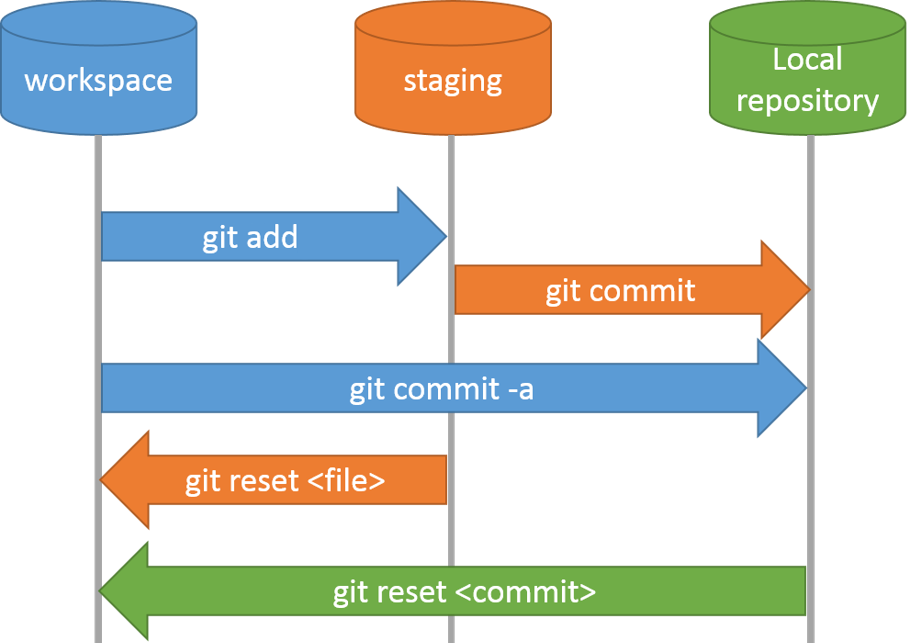
\includegraphics[height=4cm]{introduzione_a_git/git_commit_staging.png}
        \end{subfigure}
      \end{figure}
    \end{minipage}

    \subsubsection{Branch}
    Un branch è una linea di sviluppo, composta da un insieme ordinato di commit collegati in un DAG, il quale inizia dal primo commit del repository e punta all'ultimo commit.\\
    Grazie ai branch è possibile \textbf{lavorare parallelamente} a più versioni del progetto.
    \begin{figure}[H]
      \centering
      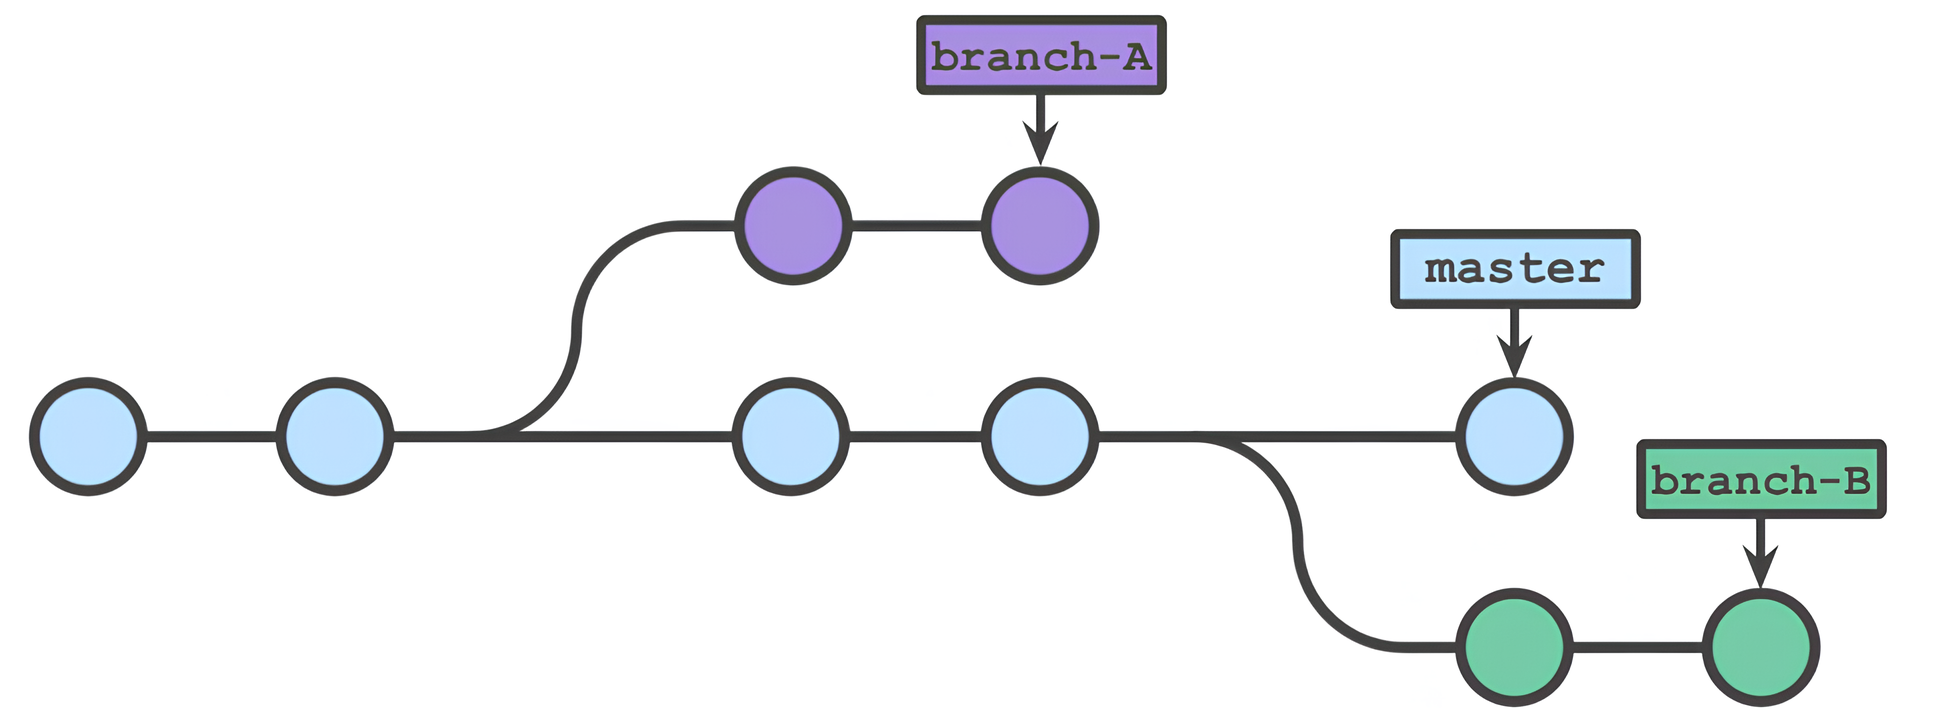
\includegraphics[width=0.7\textwidth]{introduzione_a_git/branch.png}
    \end{figure}

    \subsubsection{HEAD}
    L'HEAD è un puntatore alla posizione attuale rispetto alla storia del repository e può essere aggiornato tramite il comando \textit{checkout}.\\
    Solitamente l'HEAD punta ad un branch o ad un tag, qualora invece puntasse ad un commit si parlerebbe di \textbf{Detached HEAD}. Quando ci si trova in questo stato i commit fatti non vengono inseriti in alcun branch, rischiando quindi di andare persi.
    \begin{figure}[H]
      \centering
      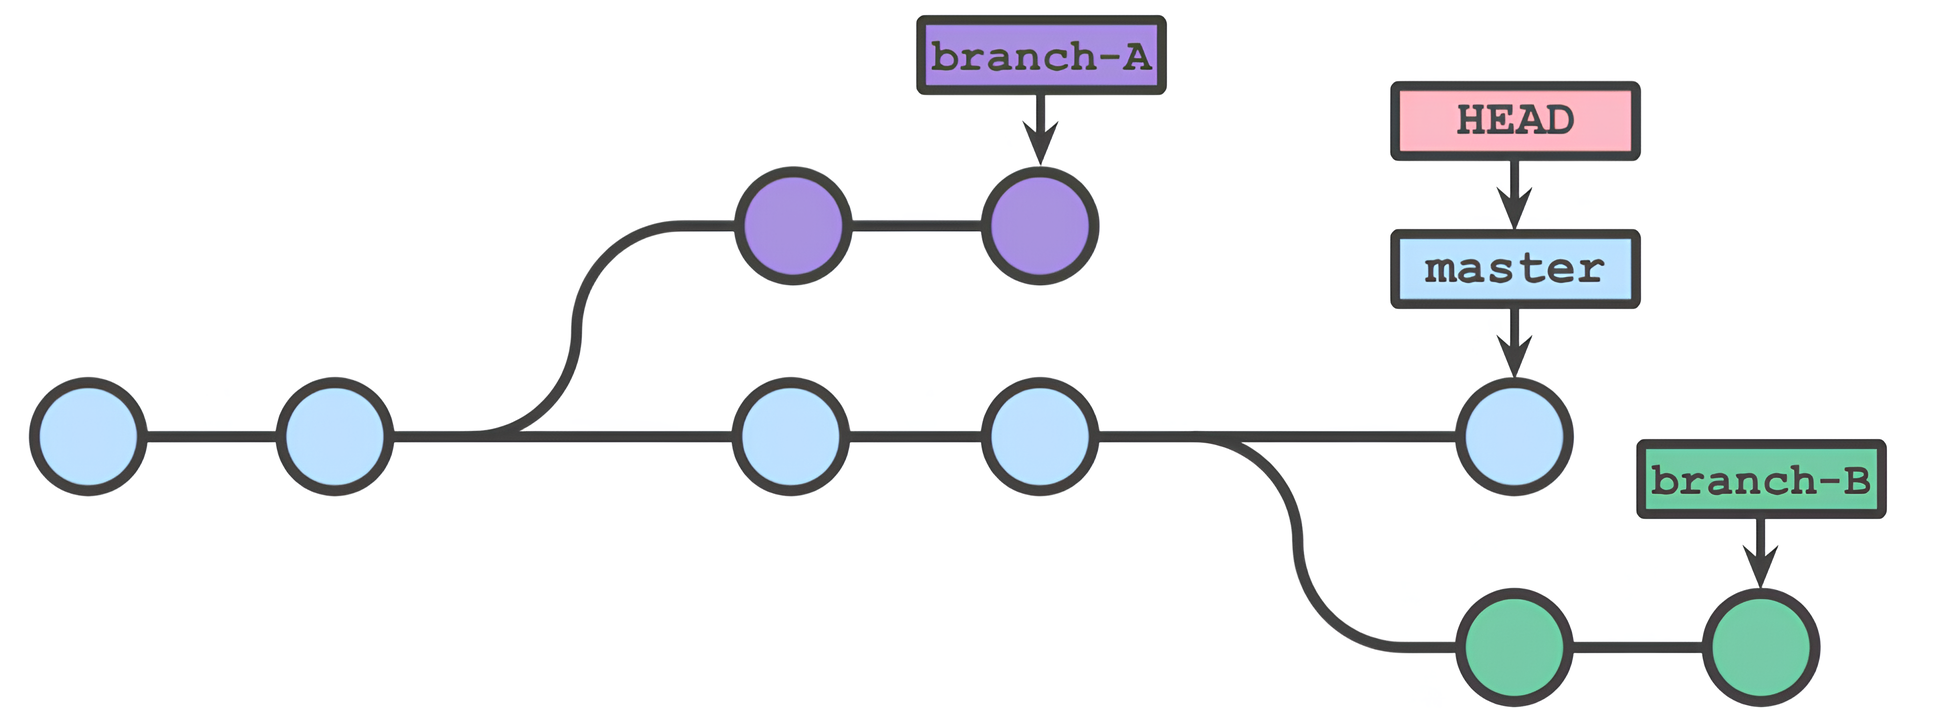
\includegraphics[width=0.7\textwidth]{introduzione_a_git/branch_head.png}
    \end{figure}

    \subsubsection{Tag}
    Un tag è un'etichetta per un commit e viene solitamente usato per segnare versioni importandi di un progetto (e.g. \textit{v1.0.0}, \textit{release-2025-09}).

    \subsubsection{Remotes}
    Sono dei riferimenti ai branch in repository remoti. Il nome predefinito è \texttt{origin} e vengono visualizzati nel formato \texttt{<remote>/<branch>} (es. \texttt{origin/main}).\\
    In particolare definiamo come \textbf{tracking branch} un branch locale che tiene traccia di un branch remoto, facilitando l'uso dei comandi \texttt{git push} e \texttt{git pull}.

    \subsubsection{Merge}
    Il merge è un'operazione che fonde i cambiamenti apportati in due branch distinti, facendo in modo che il branch di destinazione contenga entrambi i cambiamenti e che quello di origine rimanga immutato.\\
    Quando questa operazione viene eseguita tramite comando, Git determina in maniera autonoma quale tipo di merge sia più appropriato, basandosi sulla relazione tra i due branch e sullo storico dei loro commit.\\
    In particolare esistono quattro tipologie di merge:
    \begin{itemize}
      \item \textbf{Fast forward:}
        \begin{itemize}
          \item \textit{Condizione:} il branch di origine è diretto discendente di HEAD.
          \item \textit{Azione:} Git sposta solo il puntatore di HEAD in avanti. 
          \item \textit{Risultato:} nessun nuovo merge commit. 
        \end{itemize}
      \item \textbf{Merge commit:}
        \begin{itemize}
          \item \textit{Condizione:} i branch divergono e hanno sviluppi indipendenti;
          \item \textit{Azione:} Git combina le modifiche dei due branch, creando un nuovo commit;
          \item \textit{Risultato:} viene creato un merge commit con due genitori;
        \end{itemize}
      \item \textbf{Rebase:}
        \begin{itemize}
          \item \textit{Condizione:} si vuole aggiorare un branch basandolo su un altro, riscrivendo lo storico;
          \item \textit{Azione:} Git ricrea ogni commit non in comune tra i due branch; 
          \item \textit{Risultato:} la storia del branch diventa lineare, senza merge commit intermedi. 
        \end{itemize}
      \item \textbf{Three way:}
        \begin{itemize}
          \item \textit{Condizione:} storie divergenti (commit unici su entrambi i branch);
          \item \textit{Punti di confronto:}
            \begin{enumerate}
              \item Base comune (Ancestor);
              \item Versione locale (HEAD);
              \item Versione remota (Branch);
            \end{enumerate}
          \item \textit{Azione:} Git crea un nuovo snapshot combinando le modifiche;
          \item \textit{Risultato:} Viene creato un merge commit.
        \end{itemize}
    \end{itemize}

    \subsection{Comandi Git}
    Per interfacciarsi con Git vengono messi a disposizione dal sistema diversi comandi:
    \begin{itemize}
      \item \texttt{git init:} inizializza un repository creando una subdirectory .git all'interno della directory corrente; 
      \item \texttt{git status:} mostra lo stato attuale del repository (file tracciati, file modificati, file nello staging, file non tracciati);
      \item \texttt{git diff:} mostra le differenze tra working directory, staging e commit;
      \item \texttt{git add <file>:} aggiunge un file alla staging area (\texttt{git add .} per aggiungere tutti i file modificati);
      \item \texttt{git commit -m "Messaggio":} crea un commit, registrando le modifiche aggiunte con \texttt{git add} nella cronologia del repository;
      \item \texttt{git log:} mostra la lista dei commit effettuati;
      \item \texttt{git branch <nome>:} crea un nuovo branch con il nome indicato, ma \textbf{non ci si sposta};
      \item \texttt{git checkout <nome>:} passa ad un branch esistente spostando l'HEAD;
      \item \texttt{git checkout -b <nome>:} crea un nuovo branch con il nome indicato, per poi \textbf{spostarsi} su quest'ultimo (\texttt{git checkout -b <nome>} = \texttt{git branch <nome>} + \texttt{git checkout <nome>});
      \item \texttt{git fetch:} scarica gli aggiornamenti (commit, branch) dal repository remoto, \textbf{senza merge} col tuo branch;
      \item \texttt{git merge <branch>:} unisce la cronologia del branch in cui ci si trova con quella del branch specificato;
      \item \texttt{git pull:} scarica gli aggiornamenti (commit, branch) dal repository remoto, \textbf{facendo merge} col tuo branch (\texttt{git pull} = \texttt{git fetch} + \texttt{git merge});
      \item \texttt{git push:} invia i commit locali al repository remoto, aggiornando il branch remoto corrispondente; 
    \end{itemize}

    \newpage
    \subsection{Git flow}
    Con il termine Git flow intendiamo un modello di branching rigido per la gestione di rilasci e cicli di sviluppo definiti.\\
    Il suo scopo è quello di separare gli ambienti di produzione, sviluppo, funzionalità e correzioni, attraverso i seguenti branch:
    \begin{itemize}
      \item \texttt{main/master}
        \begin{itemize}
          \item \textbf{Contenuto:} solo codice stabile, testato e rilasciato.;
          \item \textbf{Checkout da:} \texttt{release-*} o \texttt{hotfix-*};
          \item \textbf{Tag:} ogni merge riceve un tag di versione (es. \textit{v1.0});
        \end{itemize}
      \begin{samepage}
        \item \texttt{develop}
          \begin{itemize}
            \item \textbf{Contenuto:} cronologia completa delle funzionalità di sviluppo;
            \item \textbf{Checkout da:} \texttt{feature-*};
            \item \textbf{Merge in:} \texttt{release-*}
          \end{itemize}
      \end{samepage}
      \item \texttt{feature-*}
        \begin{itemize}
          \item \textbf{Scopo:} lavoro isolato su una nuova funzionalità;
          \item \textbf{Checkout da:} \texttt{develop};
          \item \textbf{Merge in:} \texttt{develop};
          \item \textbf{Regola:} non interagisce mai con \texttt{main};
        \end{itemize}
      \item \texttt{release-*}
        \begin{itemize}
          \item \textbf{Scopo:} preparazione per il prossimo rilascio;
          \item \textbf{Checkout da:} \texttt{develop};
          \item \textbf{Attività:} Solo bug fixing minori e aggiornamento metadata (numero di versione);
          \item \textbf{Doppio merge in:} \texttt{main} per il rilascio in produzione e \texttt{develop} per preservare le correzioni;
        \end{itemize}
      \item \texttt{hotfix-*}
        \begin{itemize}
          \item \textbf{Scopo:} Correzione immediata di bug critici trovati nel \texttt{main};
          \item \textbf{Checkout da:} \texttt{main}
          \item \textbf{Doppio merge in:} \texttt{main} per deployare subito la correzione e \texttt{develop} per garantire che il bug non riappaia in futuro;
        \end{itemize}
    \end{itemize}

    \newpage
    \subsection{Gestione dei conflitti}
    Immaginiamo un contesto in cui tre sviluppatori lavorano allo stesso progetto:
    \begin{itemize}
      \item \textbf{Marco} (\texttt{fix-data-leakage}): si accorge di una falla critica nel preprocessing del dataset. Ha fatto 4 commit sul suo branch;
      \item \textbf{Luca} (\texttt{update-rules-parser}): ha aggiornato il parser delle regole della community, modificando gli \textbf{stessi file} di preprocessing toccati da Marco. Ha fatto 3 commit sul suo branch;
      \item \textbf{Voi} (\texttt{main}): effettuate il merge del lavoro di Marco senza problemi e ora dovete unire il lavoro di Luca.
    \end{itemize}
    Nel momento in cui proverete ad effettuare il secondo merge, Git non ve lo consentirà, mettendo in pausa il merge e marcando i file in conflitto nel seguente modo:
    \begin{lstlisting}

      <<<<<<< HEAD
      // Codice sul branch main
      =======
      // Codice sul branch update-rules-parser
      >>>>>>> update-rules-parser
    \end{lstlisting}
    A questo punto sarà necessario risolvere i conflitti tramite l'interfaccia grafica aperta dal comando \texttt{git mergetool},
    oppure manualmente aprendo ogni file, rimuovendo i marcatori di confitto e rieffettuando il commit.

    \subsection{Annullamento delle operazioni}
    \begin{itemize}
      \item \textbf{Annulare in staging:} dopo aver eseguito \texttt{git add}, qualora non si volesse più committare il file, è possibile rimuoverlo dall'area di staging tramite il comando \texttt{git reset HEAD -- <file>};
      \item \textbf{Annullare modifiche locali:} dopo aver modificato un file, è possibile scartare le modifiche e ripristinare quest'ultimo alla versione dell'ultimo commit tramite il comando \texttt{git checkout -- <file>};
      \item \textbf{Annullare un commit pubblicato:} dopo aver eseguito un commit ed averlo pubblicato, è possibile annullarlo tramite il comando \texttt{git revert <hash-commit>};
      \item \textbf{Annullare un commit locale:} dopo aver eseguito un commit, qualora quest'ultimo non sia ancora stato pubblicato, è possibile annullarlo tramite il comando\\\texttt{git reset <--soft|--hard> HEAD\raisebox{-0.5ex}{\~{}}1}, dove:
        \begin{itemize}
          \item \texttt{--soft} rimuove l'ultimo commit mantenendo le modifiche nell'area di staging;
          \item \texttt{--hard} rimuove l'ultimo commit cancellando completamente le modifiche;
          \item \texttt{HEAD\raisebox{-0.5ex}{\~{}}1} indica il commit direttamente precedente ad HEAD (\texttt{HEAD\raisebox{-0.5ex}{\~{}}3} indica il 3°, etc...); 
        \end{itemize}
      \item \textbf{Riscrivere l'ultimo commit:} per rimpiazzare l'ultimo commit con uno nuovo è possibile utilizzare il comando \texttt{git commit --amend}.
    \end{itemize}

\end{document}
